\begin{center}
    \section*{\fontsize{20}{20}\selectfont Chapter 4}
\end{center}
\vspace{10mm}

\section{Testing and System Design}
\vspace{3mm}
\large{\subsection{Testing}{Testing of an online food ordering system typically involves several stages to ensure that the system is working correctly and delivering a high-quality experience for customers. Here are some of the key steps involved in testing an online food ordering system:

\textbf{1. Unit testing:} This involves testing individual components of the system, such as the database, server-side code, and user interface elements, to ensure that they are functioning correctly.

\textbf{2. Integration testing}: This involves testing the system as a whole to ensure that all components are working together seamlessly.

\textbf{3. Functional testing:} This involves testing the system to ensure that it meets the functional requirements specified in the project scope, such as being able to search for restaurants, view menus, place orders, and track deliveries.

\textbf{4. Performance testing:} This involves testing the system to ensure that it can handle high volumes of traffic and orders without slowing down or crashing.

\textbf{5. Security testing:} This involves testing the system to ensure that it is secure and protected against common vulnerabilities, such as SQL injection attacks or cross-site scripting (XSS) attacks.

\textbf{6. User acceptance testing:} This involves testing the system with real users to ensure that it is easy to use, meets their needs, and delivers a high-quality experience.

Overall, testing is a critical part of the development process for an online food ordering system, helping to ensure that it is reliable, secure, and user-friendly.}}


{\subsection{System Design}
{System design for an online food ordering system:
\begin{figure}[h]
    \centering
    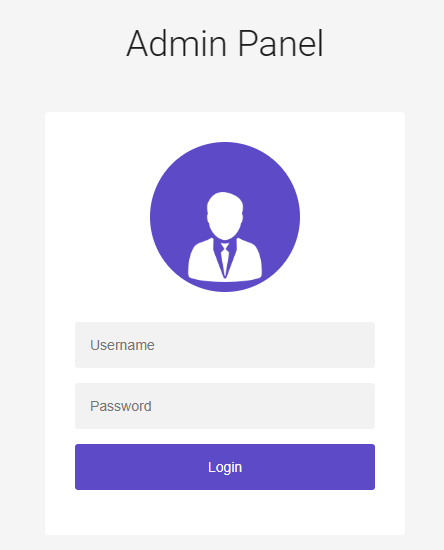
\includegraphics[scale=0.55]{admin1.png}
    \caption{Admin Login Page}
    \label{fig.a}
\end{figure}\begin{figure}[h]
    \centering
    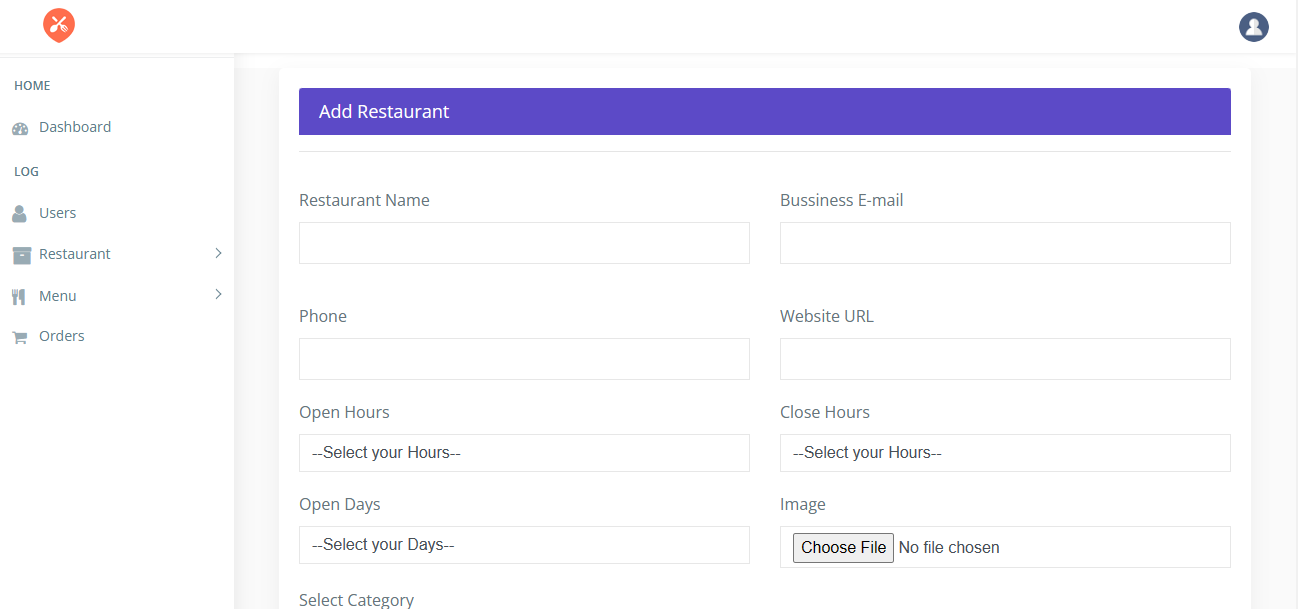
\includegraphics[scale=0.55]{admin2.png}
    \caption{Admin Page}
    \label{fig.b}
\end{figure}\begin{figure}[h]
    \centering
    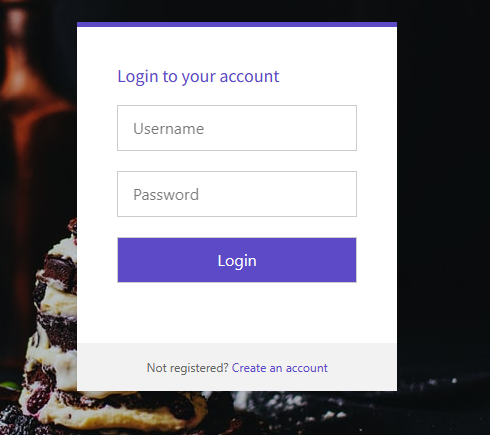
\includegraphics[scale=0.55]{user1.png}
    \caption{User Login Page}
    \label{fig.c}
\end{figure}\begin{figure}[h]
    \centering
    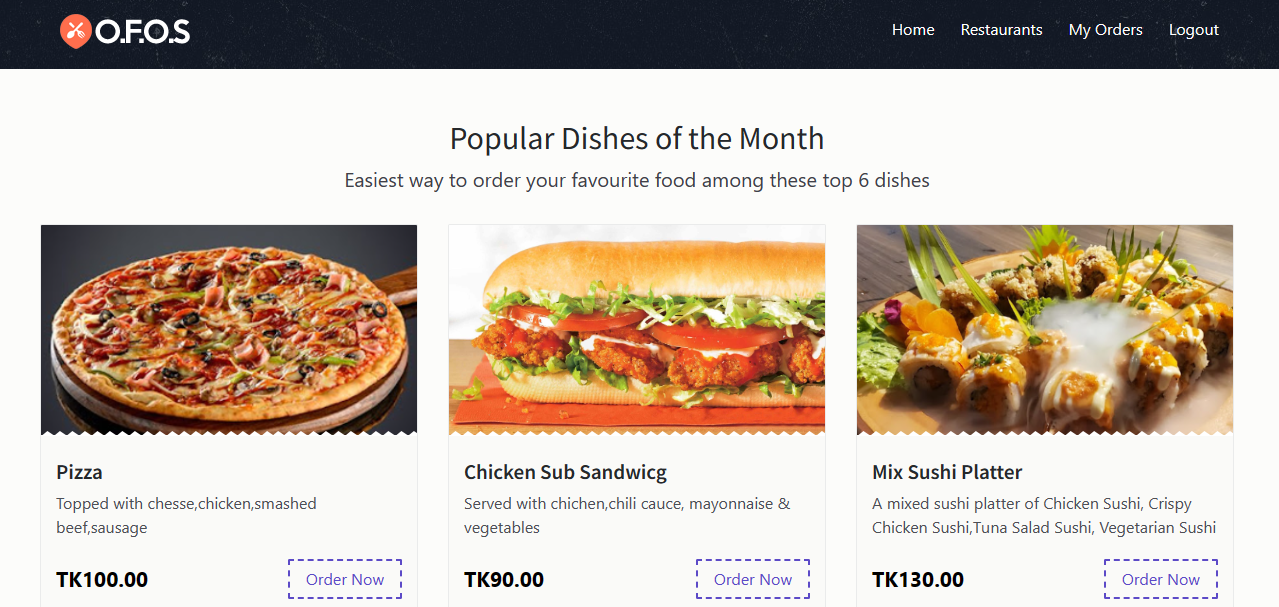
\includegraphics[scale=0.55]{user2.png}
    \caption{Home Page}
    \label{fig.d}
\end{figure}\begin{figure}[h]
    \centering
    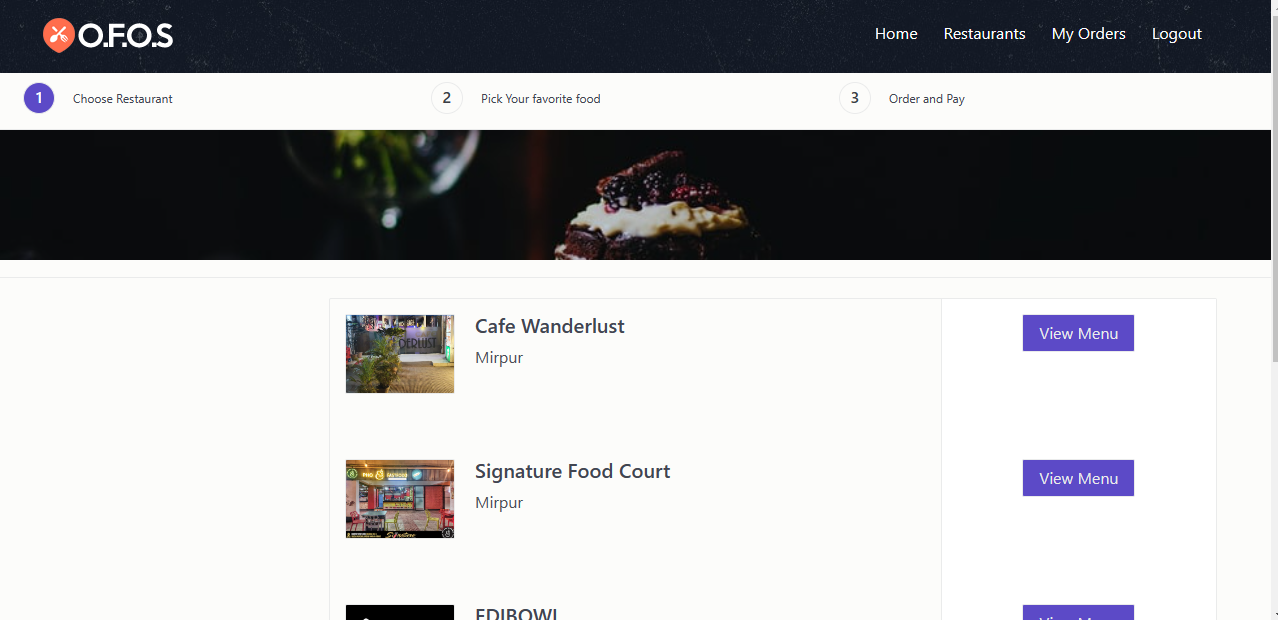
\includegraphics[scale=0.55]{user3.png}
    \caption{Restaurant page}
    \label{fig.e}
\end{figure}\begin{figure}[h]
    \centering
    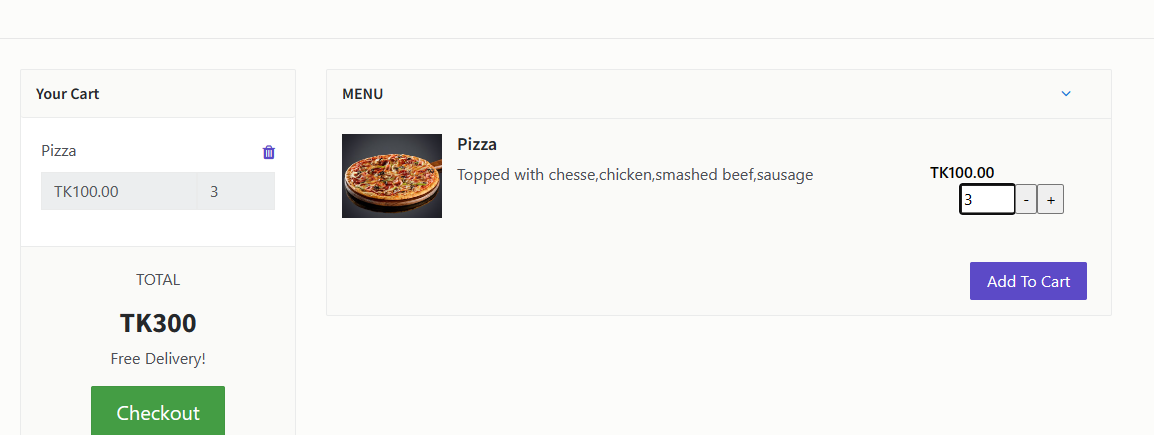
\includegraphics[scale=0.55]{user4.png}
    \caption{My Order}
    \label{fig.5}
\end{figure}\begin{figure}[h]
    \centering
    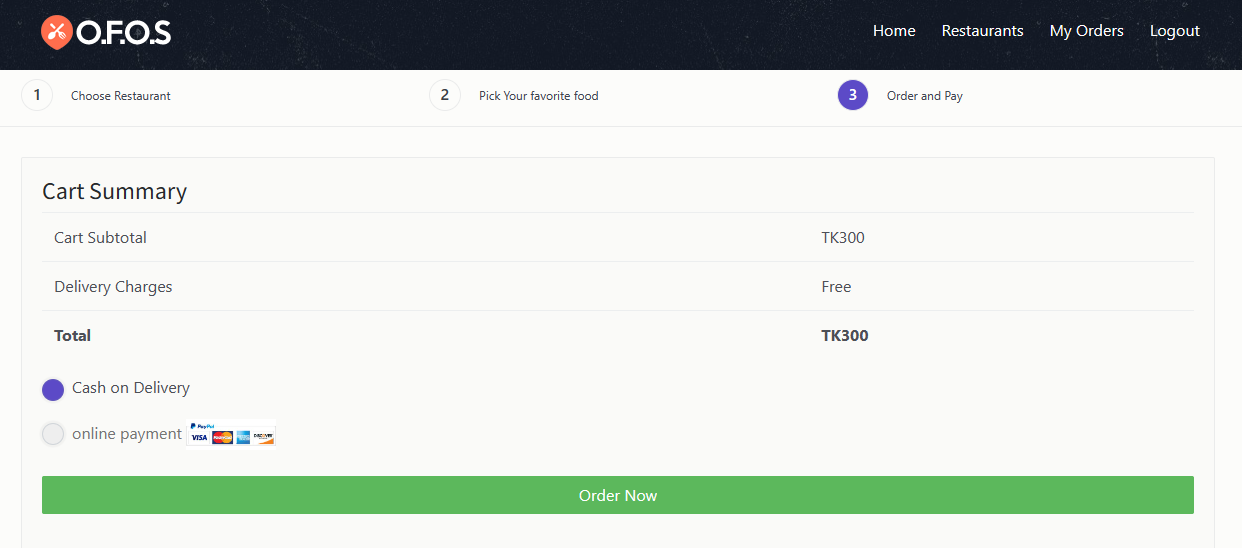
\includegraphics[scale=0.55]{user5.png}
    \caption{Payment method}
    \label{fig.5}
\end{figure}}}

